\documentclass[12pt]{article}
\usepackage[utf8]{inputenc}
\usepackage{graphicx}
\usepackage{hyperref}
\usepackage{amssymb}
\usepackage{amsmath}
\usepackage[T1]{fontenc}
\usepackage{lmodern}
\usepackage{textcomp}
\usepackage{pgfplots}
\usepackage{pgfplotstable}
\usepackage{longtable}
\usepackage[capitalise]{cleveref}
\usepackage{caption}
\pgfplotsset{compat=1.18}
\captionsetup[table]{position=top,justification=raggedright,singlelinecheck=false}
\captionsetup[longtable]{position=top,justification=raggedright,singlelinecheck=false}
\captionsetup[figure]{justification=raggedright,singlelinecheck=false}
\setlength\LTleft{0pt}
\setlength\LTright{0pt}
\setlength\LTcapwidth{\textwidth}
\pgfplotstableset{
  show variable once/.style={
    columns/variable/.style={
      string type,
      column name=Variable,
      postproc cell content/.code={
        \pgfkeysgetvalue{/pgfplots/table/@cell content}{\cellcontent}
        \edef\currentvar{\cellcontent}
        \ifx\currentvar\lastvar
          \pgfkeyssetvalue{/pgfplots/table/@cell content}{}
        \else
          \ifnum\pgfplotstablerow>0
            \pgfkeyssetevalue{/pgfplots/table/@cell content}{\noexpand\hline\space\cellcontent}
          \fi
          \xdef\lastvar{\currentvar}
        \fi
      }
    }
  }
}
\def\lastvar{}
\setlength{\parskip}{0.8em}
\setlength{\parindent}{0pt}
\newcommand{\indep}{\perp \!\!\! \perp}

\title{\Large\bfseries ASSIGNMENT 6: MARGINAL MODELS (GEE)}
\author{Chenghao Wang}
\date{\today}

\begin{document}

\maketitle

\section{Model Specification}

\subsection{Outcome and link function}

The outcome is \texttt{PreBD\_FFB} whose value is 
either "obstruction" (obstructive ventilatory defect) or "normal".
We define a binary outcome
\[
Y_{ij} = I(\texttt{PreBD\_FFB}_{ij} = \text{obstruction}),
\]
where $Y_{ij}=1$ indicates obstruction for subject $i$ at visit $j$.
Because the outcome is binary, we use a logit link and Bernoulli variance
function:
\[
\mathrm{logit}(\mu_{ij}) =
\log\left(\frac{\mu_{ij}}{1-\mu_{ij}}\right), \qquad
\mathrm{Var}(Y_{ij}) = \mu_{ij}(1-\mu_{ij}),
\]
where $\mu_{ij}=P(Y_{ij}=1)$ is the marginal probability of obstruction.
This model gives population-averaged effects on the log odds of obstruction.

\subsection{Mean model}

To specify the marginal mean model, we made a plot 
of $\mathrm{logit}(\hat{P}(Y_{TG,j} = 1))$, where
$\hat{P}(Y_{TG,j} = 1)$ is the observed probability of obstructuion
for subjects in group TG at visit $j$, as shown in \cref{fig:prebd-ffb-logit-all}.
Our dataset contains high missingness in
\texttt{PreBD\_FFB} at some time points
which appears to introduce considerable bias.
Thus, time points with more than 75\% missingness in
\texttt{PreBD\_FFB} were removed, which were visits 44, 56, 64, and 120.
The observed logits after removing these visits are shown in
\cref{fig:prebd-ffb-logit-le75}. The trend between the observed logits and visit times
appear non-linear and fluctuates wildly, so we selected a saturated marginal mean structure.

The marginal mean model is
\begin{equation}
\mathrm{logit}(\mu_{ij})
= \beta_0 + TG_i + visit_j + TG_i:visit_j
+ age\_rz_i + gender_i + ethnic_i.
\end{equation}

$\beta_0$ represents the intercept. Treatment group, visit time, gender, and ethnicity are modeled as categorical
variables, while age at randomization is modeled as a continuous variable.
The treatment-by-visit interaction allows the population-averaged trajectory
to differ by treatment group.


\begin{figure}[htbp]
\centering
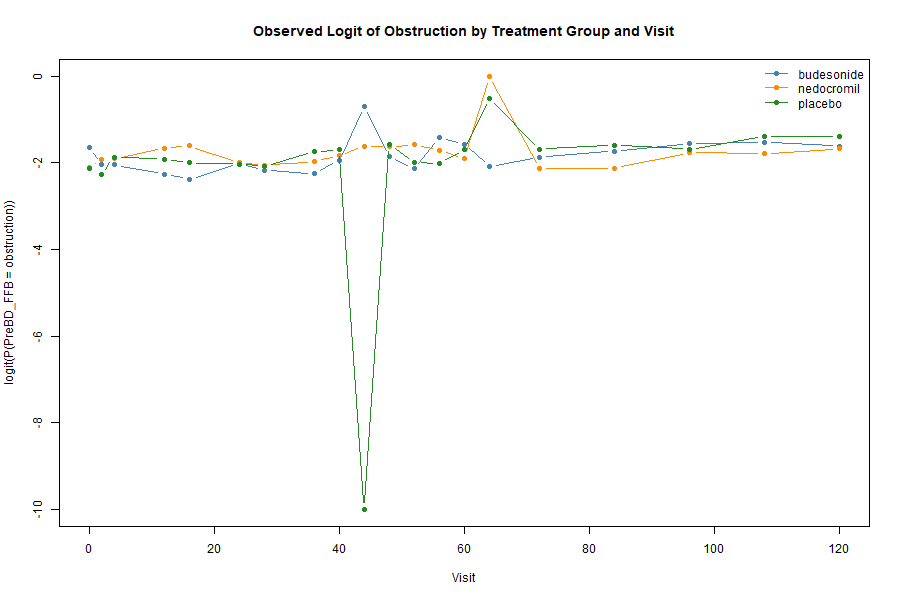
\includegraphics[width=0.85\textwidth]{../hw6_code/output/prebd_ffb_logit_by_tg_visitc.png}
\caption{Observed logit of pre-bronchodilator obstruction by treatment group and visit.}
\label{fig:prebd-ffb-logit-all}
\end{figure}

\begin{figure}[htbp]
\centering
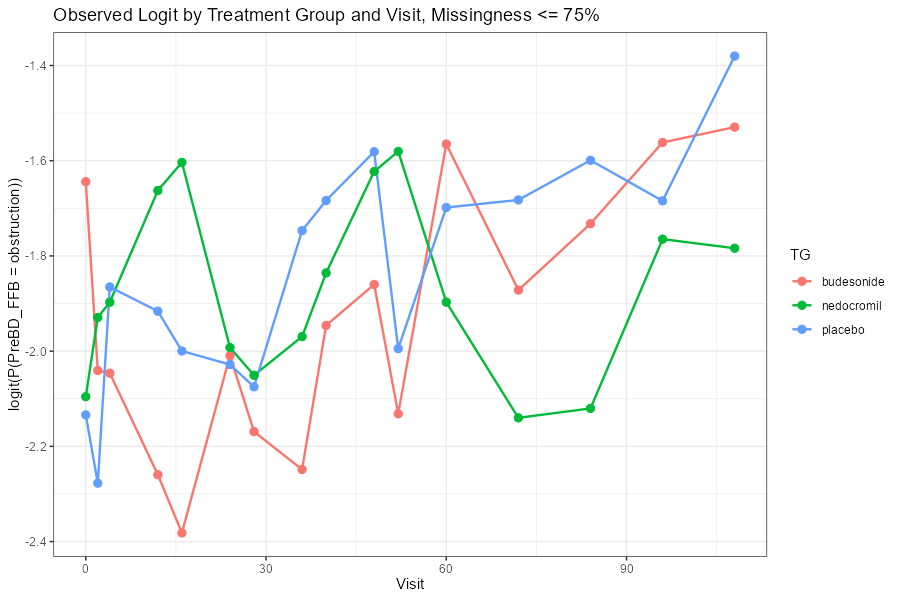
\includegraphics[width=0.85\textwidth]{../hw6_code/output/prebd_ffb_logit_by_tg_visitc_missingness_le75.png}
\caption{Observed logit of pre-bronchodilator obstruction after removing visits with more than 75\% missingness.}
\label{fig:prebd-ffb-logit-le75}
\end{figure}

\section{Working Correlation Structure}

\subsection{Fitting the model}

The GEE model was fitted using independence and AR(1) working correlation
structures. 
The R package \texttt{geepack} was used.
The coefficient estimates from both fits are shown in
\cref{tab:gee-parameter-estimates}.

\begingroup
\small
\pgfplotstabletypeset[
  col sep=comma,
  string replace*={"}{},
  string replace*={_}{\_},
  begin table=\begin{longtable},
  end table=\end{longtable},
  every head row/.style={
    before row={\caption{GEE coefficient estimates under independence and AR(1) working correlation structures.}\label{tab:gee-parameter-estimates}\\\hline},
    after row=\hline
  },
  every last row/.style={after row=\hline},
  display columns/0/.style={string type, column name=Parameter, column type=p{0.46\textwidth}},
  display columns/1/.style={column name=Independence, column type=r, fixed, precision=3},
  display columns/2/.style={column name=AR(1), column type=r, fixed, precision=3}
]{../hw6_code/output/gee_parameter_estimates.csv}
\endgroup

\subsection{Comparing structures}

The parameter estimates were broadly similar under the two working correlation
structures. We used QIC to select the working correlation structure, 
which is analogous to AIC but uses quasi-likelihood.
The independence model had QIC 7674.8, while the AR(1) model had
QIC 7693.5. Since smaller QIC is preferred, the independence working
correlation was selected for the remaining inference.

\section{Variance Estimation}

\subsection{Comparison}

For the selected independence working correlation structure, the model-based
and sandwich standard errors are demonstrated in \cref{tab:gee-se-comparison}.


\begingroup
\small
\pgfplotstabletypeset[
  col sep=comma,
  string replace*={"}{},
  string replace*={_}{\_},
  begin table=\begin{longtable},
  end table=\end{longtable},
  every head row/.style={
    before row={\caption{Model-based and sandwich standard errors for the independence GEE fit.}\label{tab:gee-se-comparison}\\\hline},
    after row=\hline
  },
  every last row/.style={after row=\hline},
  display columns/0/.style={string type, column name=Parameter, column type=p{0.46\textwidth}},
  display columns/1/.style={column name=Model-based SE, column type=r, fixed, precision=3},
  display columns/2/.style={column name=Sandwich SE, column type=r, fixed, precision=3}
]{../hw6_code/output/gee_independence_se_comparison.csv}
\endgroup

\subsection{Interpretation}
Discrepancies exist between the two sets of standard errors,
of which the direction is not consistent across the parameters.
Some sandwich standard errors differ markedly from the model-based standard
errors, especially for baseline covariates such as age, gender, and ethnicity.
In longitudinal data analysis, it is usually unreasonable to assume
no within-subject correlation.
Thus we use the sandwich standard errors for inference
because they are robust to misspecification of the working correlation in GEE.

\section{Hypothesis Testing and Interpretation}

\subsection{Hypothesis test}

To evaluate whether the population-averaged log odds of obstruction 
(More precisely, it is logit of the population-averaged probability of obstruction)
trajectories differs by
treatment group, we tested
\[
H_0:\ \text{all treatment-by-visit interaction coefficients are zero}
\]

against the alternative that at least one treatment-by-visit interaction is
nonzero. 

The Wald test statistic is 46.55 with 30 degrees of freedom, and the p-value is
0.028. Thus, we reject the null hypothesis at the 0.05 level and conclude that
the population-averaged log odds of obstruction trajectories differ by treatment group.


\subsection{Interpretation of effects}

For this binary outcome with a logit link, exponentiated parameters estimates 
would be
interpreted as odds ratios at the population-level. 
However, because the mean model
uses a saturated structure, the parameter estimates are hard to interpret directly.

\section{Summary}

We fit a marginal logistic model using GEE 
with an independence working correlation matrix.
There is evidence that the population-averaged log odds of obstruction trajectories
differs by
treatment group. The model is useful for estimating marginal (population level) treatment-group
patterns, but it has limitations. 
First, it does not provide subject-specific estimates.
Besides, it requires the strong assumption of MCAR.
Lastly, our model has too many parameters, which makes the
interpretation difficult.

\section{Code Availability}

The code is available at
\url{https://github.com/CHENGHAO-WANG/767_homework/tree/main/hw6_code}.

\end{document}
